\chapter{Implementation}
\label{ch:implementation}


In this chapter, a concrete implementation of the proposed approach is discussed. 
Details about significant methods and practical use cases of RDF-Doctor  are presented in the following.  
 
%\section {Architecture}

%The design of the architecture is planned based on the Input-Process-Output Model. 
%It can be also considered as a black-box solution where the solution processes the input, then it delivers the output once it is ready.\todo{the description of the architecture is almost the same as described in the approach} 
%The architecture is composed of three main phases as described in Figure \ref{Fig:Architecture}:



%\begin{itemize}
% \item \textbf {Input}: It is the role of the user to provide an RDF file with certain options, such as 1) enabling/disabling of the error correction; 2) showing an error report of JSON\footnote{https://www.json.org/} or text format; and 3) concealing/showing up the parse tree.
 
%\item \textbf{Processing}: starts with preparing the input to be parsed in the following workflow: 1)it reads the input; 2) splits it into smaller pieces if needed; 3) parses the input for each slice (if many); and 4) corrects a subset of detected syntax errors. 
%This phase utilizes the parser built based on a predefined grammar.
%it requires ANTLR library for parsing, and some options from the user to activate/deactive some features of the solution.   
%\item \textbf{Output}: provides the reports after processing phase, %including 1) an error report to announce the detected syntax errors; 2) a correction report which lists the recovered syntax errors; and 3) an output file after healing some of the detected syntax errors\todo{It is not clear what is the point number 3}; and 4) a frame contains the parse tree. 
%Both, the correction report and the output file require to be enabled in order to be generated. 
%\end{itemize}

%\section {Modules} change Modules to Methods is a good idea

\section {Methods} 

%After briefing the proposed solution architecture, It is the time to cover it in more details by shedding light onto those modules which represent the pillars of such solution.
The implementation of RDF-Doctor is composed of several modelus.
{Figure~\ref{Fig:UML}} illustrates a UML diagram of the three most important methods: Main, Error Detection, and Error Correction. 
The following text discusses these methods in detail as well as so-called the Core module.%, which is not shown in the diagram to avoid the complexity of description.
%It is worth to be noted that Core module is not shown in {figure \ref{Fig:UML}} to facilitate the understanding of the main modules, otherwise it would be complex,
%Core is automatically generated module by ANTLR based on the given grammar, thereby few changes were coded in the module:  

	\begin{figure}[ht]
	\begin{center}
		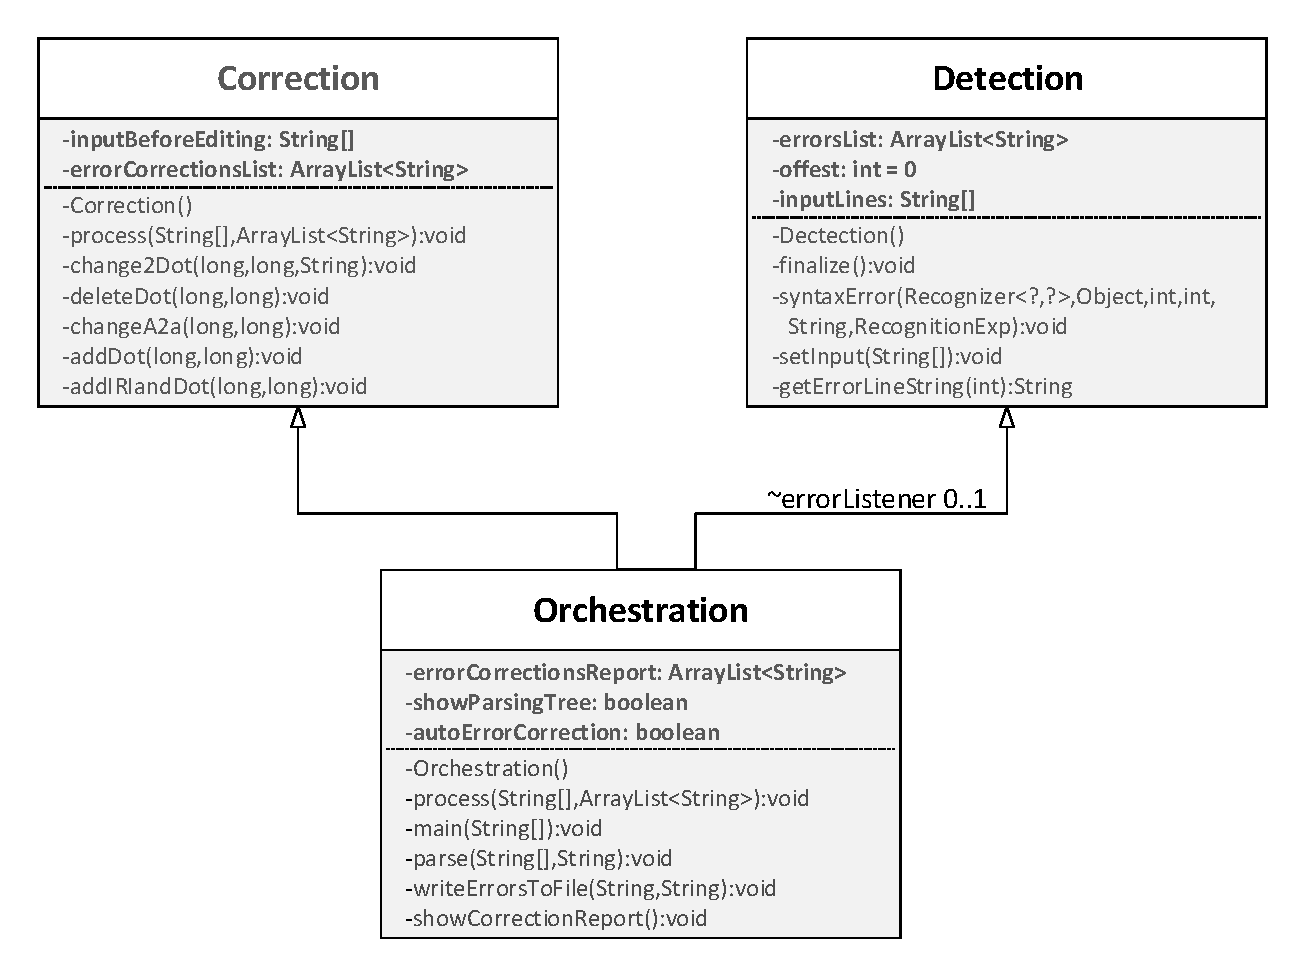
\includegraphics[scale=0.65,angle=0]{images/methods.pdf}
		\setlength{\abovecaptionskip}{0pt} 
				\setlength\belowcaptionskip{-5mm}
		\caption{\textbf{Components of RDF-Doctor.} 
		Three main components of RDF-Doctor. 
		Orchestration Module parses RDF input and encountered errors are collected by \emph{errorListener}.
		The \emph{errorDetection} method handles errors collected in errorlistener and releases the appropriate error messages.
		Finally, the errorCorrection method perform recovery actions to certain errors.}
		\label{Fig:UML}
	\end{center}
\end{figure}
%TODO:check here how to adjust the vertical space 


\begin{enumerate}[]
 \item \textbf {Core}: is automatically generated by ANTLR based on the predefined grammar, which is listed in Appendix~\ref{ch:appendix}. 
 It encloses parsing classes, such as Parser, Lexer, Error Collector, Parse Tree Creator.   
\item \textbf{Errors Detection}: listens to the generated error messages by the parser. 
Commonly, during parsing procedure, if the parser detects syntax errors it sends a notification an error listener, if one was defined. 
This module enriches the list of errors that are collected by the error listener with valuable information about the errors, such as an expressive message to describe the actual error, an error location, identified by line and column numbers, and sometimes the actual line text where the parser has discovered a particular error.

\item \textbf {Error Correction}: corrects those syntax errors which have a known solution. 
The error message plays an important role to identify whether such error can be corrected or not. 
A global list stores all detected syntax errors, including their messages and location in the input file. % (line number and column number) and this modules has predefined messages. 
If any of the detected error messages matches any of the predefined messages, then such error can be recovered.

\item \textbf{Orchestration}: \todo{Maybe rename this module, instead of Main to "Orchestration", dont forget also in the Diagram} is the executive part which combines input, output, and processing components. 
It receives the input text, and if it is large (for example, more than 1 million lines), it is splits chunks according to a predefined size. 
Each chunk is handled separately with regard to parsing, error detection, as well as error correction.

\end{enumerate} 


\section{Use Cases in Practice}
In this section, some of use cases tackled in this study to detect syntax errors and correct some of the detected syntax errors are elaborated. 
First, we start with a Turtle example which has no syntax errors, then some syntax errors are introduced to show the process of handling them. 

%\vspace{5mm} %5mm vertical space

Listing \ref{lst:turtleExample} shows a Turtle example without syntax errors. 
The first four lines are directives or prefixes declaration whereas in the rest of lines several triples are listed.  
For that reason, our grammar in Appendix~\ref{ch:appendix} is initialized with the topmost node \textbf{start} which describes the coming rules by zero or more  \textbf{statement}(s). 
In addition, each \textbf{statement} is either a directive or a triple as it is represented in \ref{lst:startingRules}.

\begin{lstlisting}[label=lst:startingRules, caption={Starting rules in the grammar file}] 
start
: statement*  EOF
;
statement
: directive
| triples '.'
\end{lstlisting}

\begin{lstlisting}[label=lst:turtleExample, numbers=left, caption={RDF example in Turtle serialization format}]
<@\textcolor{blue}{@prefix}@>  <@\textcolor{red}{rdf}@>: <@\textcolor{orange}{<http://www.w3.org/1999/02/22-rdf-syntax-ns\#>}@> .
<@\textcolor{blue}{@prefix}@>  <@\textcolor{red}{rdfs}@>:  <@\textcolor{orange}{<http://www.w3.org/2000/01/rdf-schema\#>}@> .
<@\textcolor{blue}{@prefix}@>  <@\textcolor{red}{ex}@>:  <@\textcolor{orange}{<http://example.org/>}@> .
<@\textcolor{blue}{@prefix}@>  <@\textcolor{red}{zoo}@>:   <@\textcolor{orange}{<http://example.org/zoo/> }@> .
<@\textcolor{red}{ex}@>:dog1  <@\textcolor{red}{rdf}@>:type  <@\textcolor{red}{ex}@>:animal .
<@\textcolor{red}{ex}@>:cat1  <@\textcolor{red}{rdf}@>:type  <@\textcolor{red}{ex}@>:cat ;
         <@\textcolor{red}{rdfs}@>:label   <@\textcolor{green}{"Lusi"@en}@> .
<@\textcolor{red}{ex}@>:cat  <@\textcolor{red}{rdfs}@>:subClassOf  <@\textcolor{red}{ex}@>:animal .
<@\textcolor{red}{zoo}@>:host  <@\textcolor{red}{rdfs}@>:range  <@\textcolor{red}{ex}@>:animal .
<@\textcolor{red}{ex}@>:zoo1  <@\textcolor{red}{zoo}@>:host  <@\textcolor{red}{ex}@>:cat2 .
\end{lstlisting}



\begin{figure}
		\centering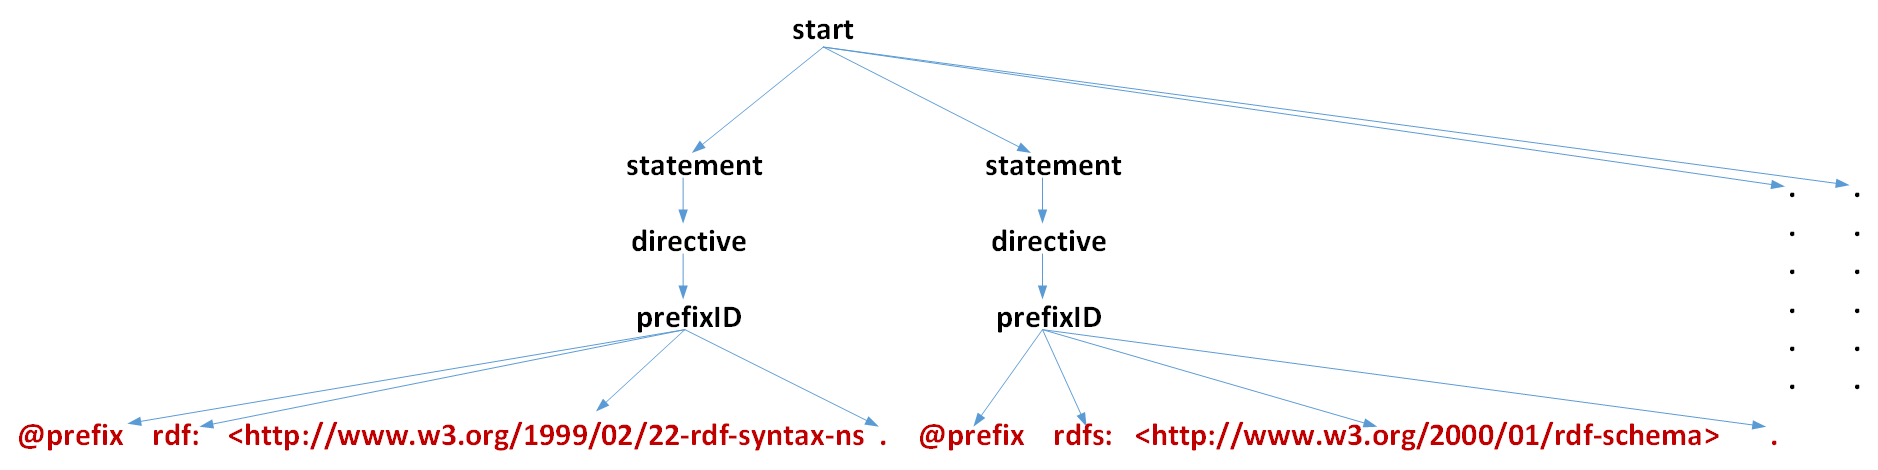
\includegraphics[width=1.12\linewidth]{images/implementationParseTreeLeft.png}
		\caption{\textbf{Left-side parse tree view of Listing~\ref{lst:turtleExample}.} The view shows left-side sub-trees of the parent node start of the parse tree and it also demonstrates the hierarchy of applying grammar rules where all nodes written in black are non-terminals or heads of the grammar rules, remaining nodes are terminals or matched patterns of input tokens.}
	\label{Fig:implementationParseTreeLeft}
\end{figure}

\begin{figure}
		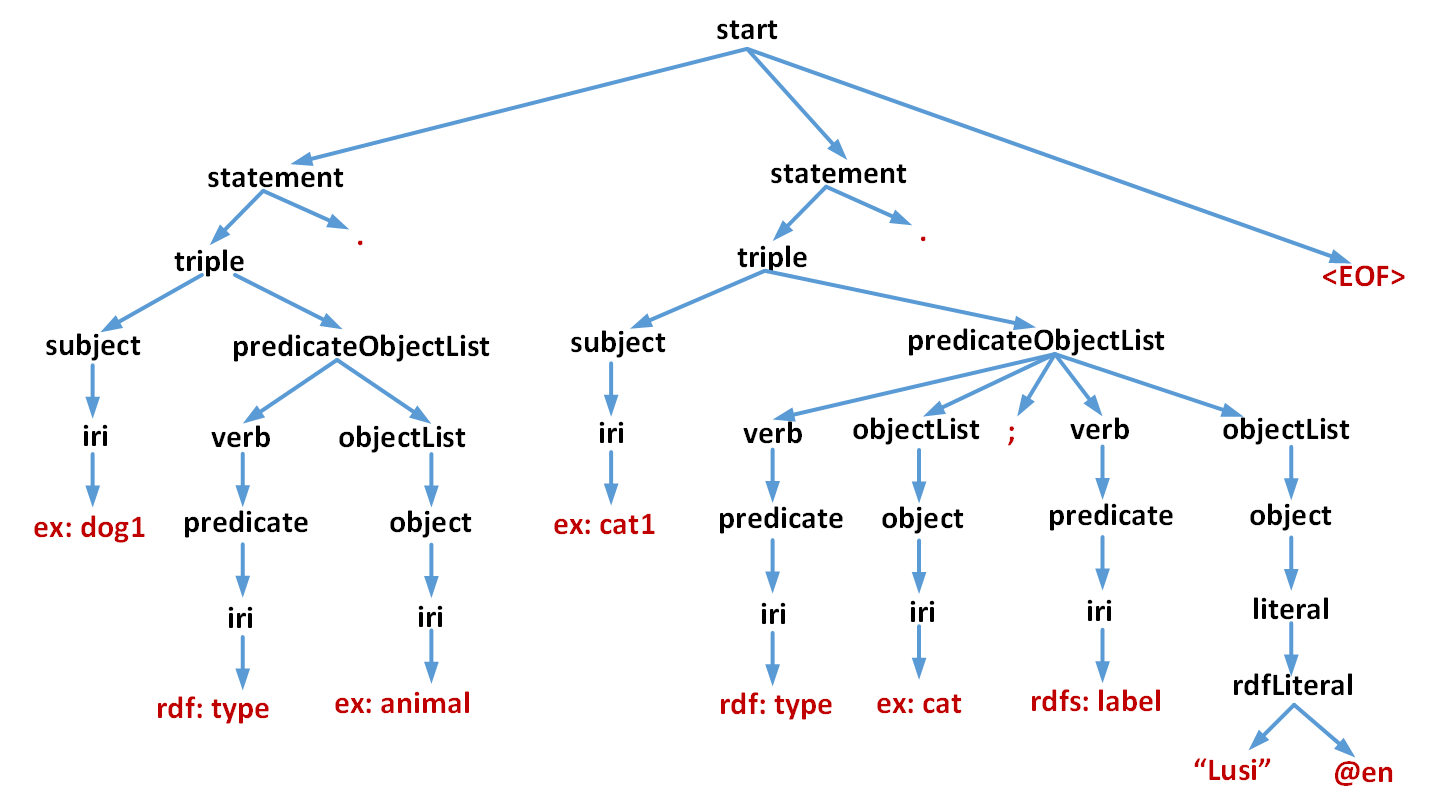
\includegraphics[width=1\linewidth]{images/implementationParseTreeRight.png}
	\caption{\textbf{The right-side parse tree view of listing \ref{lst:turtleExample}.} It is right-side sub-trees of the parent node \textbf{start} in the parse tree.}
	\label{Fig:implementationParseTreeRight}

\end{figure}

After showing a part of grammar rules and views of the parse tree, some of real cases of handling error detection and error recovery will be presented:

\begin{enumerate}
    \item \textbf{Missing a dot at the end of a triple:} in the Turtle syntax, a triple must end with a dot. 
    In Listing~\ref{lst:missingDotEx}, the head rule, i.e., a \textbf{statement}, can either be a directive or a triple, both ending with a dot. 
    Equally important the last line which shows that triples without a dot can also be a sub-goal of this rule. 
    This sub-goal is considered as a normal path in a parse tree, but once the parser detects it, it sends a notification to the error listener with an error message \emph{"Missing ’.’ at the end of a triple"}.  
    
    
\begin{lstlisting}[label=lst:missingDotEx,  caption={The grammar rule for Detection of a syntax error for a missing dot at the end of a triple.}] 
statement
: directive
| triples '.'
| <@\textcolor{red}{triples  \{notifyErrorListeners("Bad end of a triple
               with ','")\} }@>;
\end{lstlisting}
Once such error is saved by the Error Listener, the role of Error Detection Module is finished. 
The next is the phase starts in the Error Correction Module to correct the error. 
Since the list of syntax error is shared with Error Correction Module, it iterates all of these errors messages, if one of these messages in the error list matches, then it applies a predefined function to recover the error.  
For instance, \textbf{addDot(lineNum, columnNum)} function is applied, as described in Listing \ref{lst:errorCorrectionlst}, since it matches the same error message and similarly, in case of \emph{"Missing  ’.’ at the end of Prefix directive"} message. 
The task of this function is to reach the line which misses the dot, identify the lineNum and columNum values automatically correct the error by adding a dot in the end of the given triple. 

\begin{lstlisting}[language=java, label=lst:errorCorrectionlst,  caption={Java-based handling for error recovery based on the error message in Error Correction Module.}] 

while (iterator.hasNext()) {
String line = iterator.next();
// select the action based on the error message
if (line.contains("Missing '.' at the end of Prefix
directive")||line.contains("Missing '.' at the end 
of a triple"))
<@\textcolor{violet}{addDot(lineNum, columnNum);}@>
else if (line.contains("'A' cannot be used as
predicate, it should be repalced with 'a'"))
<@\textcolor{violet}{changeA2a(lineNum, columnNum);}@>
}
\end{lstlisting}

\item \textbf{Misuse of 'A' as a predicate instead of 'a':} by mistake a user can wrongly use the character 'A' as a predicate instead of using 'a', which is the short version of the \emph{rdf:type}%, to ease its usage, it was replaced with 'a'). 
If we start substitution of sub-goals of triples, \textbf{verb} can be found as a terminal node in  substitution chain. 
Syntactically, it is 'a', but if the user used 'A', then the parser will fire an error with a message "’A’ cannot be used as a predicate, it should be replaced with ’a’".
Listing \ref{lst:errorCorrectionlst} also shows the handling of this error by executing \textbf{changeA2a(lineNum, columnNum)} function where the same error message is matched. 
This function can access Turtle input with the referred lineNum and columNum, then it replaces 'A' with 'a' to correct that error. 

\begin{lstlisting}[label=lst:MissuseAex ,  caption={The grammar rule for detecting the misuse of 'A' as a predicate instead of 'a' in the grammar.}] 
statement
: directive
| triples '.';
triples
: subject predicateObjectList;
predicateObjectList
: verb objectList (';' (verb objectList)?)*;
verb
:'a'
| <@\textcolor{red}{'A' {notifyErrorListeners("'A' cannot be used as
predicate, it should be replaced with 'a'");}}@>;
\end{lstlisting}

\item \textbf{Bad syntax of a language tag in a literal:} 
Turtle formats has the ability to specify the language of a literal (which can be only placed as an object) by the using the character '@' followed by alphabetic characters, for example, "en", "fr", "de" are tags for English, French, German languages, respectibely. 
\textbf{"Cat"@en}, and \textbf{"Katze"@de} are some examples of literals which use the language tags.

\begin{lstlisting}[label=lst:badlaguageTag,  caption={Starting rules in the grammar file8}] 
triples
: subject predicateObjectList;
predicateObjectList
: verb objectList (';' (verb objectList)?)*;
objectList
: object (',' object)*
object
: literal;
literal
: rdfLiteral;
rdfLiteral
: String (LANGTAG | '^^' iri)?
| <@\textcolor{red}{ String  BAD\_LANGTAG\_AS\_NUMBER  {notifyErrorListeners("Language tag cannot be a numeric value");} }@>;
BAD_LANGTAG_AS_NUMBER : 
'@' [0-9]+;
\end{lstlisting}

It might happen that a user instead of providing a language tag for a literal, he or she wrongly types a number, such as \textbf{"cat"@1}.
This should be considered as a syntax error in Turtle format. 
Listing~\ref{lst:badlaguageTag} handles the sequence of rules in the grammar to make a parser firing a syntax error when such case is encountered. 
The hierarchical structure of the rules can be traversed, starting with \textbf{triples} head rule until it reaches the last two lines.
It specifies that an RDF literal can be a string followed by BAD\_LANGTAG\_AS\_NUMBER (which '@' character followed by numbers). 
When the parser finds such a pattern in the input, it delivers a syntax error to the error listener. 
Unfortunately, no error correction can be applied here, since the user intention is not easily known.  

\end{enumerate}
